\chapter{Theoretical Background} 	% Produces section heading.  Lower-level

%Basics such as theory, definitions, relevant theories, related work and state of the art should be included here.

TODO

% TODO: maximal 1.1.1 
% TODO: wenns 1.1 gibt, muss es auch 1.2 geben

\section{General Definitions}
\label{theoretical-background:general-definitions}

The following section includes general definitions of terms on the topic.

\subsection*{Cloud Computing}

\begin{quotation}
\noindent
\enquote*{Cloud computing is a model for enabling ubiquitous, convenient, on-demand network access to a shared
	pool of configurable computing resources (e.g., networks, servers, storage, applications, and services) that
	can be rapidly provisioned and released with minimal management effort or service provider interaction.
	This cloud model is composed of five essential characteristics, three service models, and four deployment
	models.}
\autocite{cloudComputingNistDefinition2011}
\end{quotation}

The characteristics are
\autocite{cloudComputingNistDefinition2011}:

\begin{itemize}
	\item On-demand self-service
	\item Broad network access
	\item Resource pooling
	\item Rapid elasticity
	\item Measured service
\end{itemize}

The service models are
\autocite{cloudComputingNistDefinition2011}:

\begin{itemize}
	\item Software as a Service (SaaS)
	\item Platform as a Service (PaaS)
	\item Infrastructure as a Service (IaaS)
\end{itemize}

The deployment models are
\autocite{cloudComputingNistDefinition2011}:

\begin{itemize}
	\item Private cloud
	\item Community cloud
	\item Public cloud
	\item Hybrid cloud
\end{itemize}

\subsection*{Cloud Native Application}

\begin{quotation}
\noindent
\enquote*{A cloud-native application (CNA) is a distributed, elastic and horizontal scalable system composed of (micro)services which isolates state in a
minimum of stateful components. The application and each self-contained
deployment unit of that application is designed according to cloud-focused
design patterns and operated on a self-service elastic platform.}
\autocite{cloudNativeApplicationDefinition2017}
\end{quotation}

\subsection*{Continuous}
\begin{quotation}
\noindent
\enquote*{"Continuous" is intended to match the industry standard term: reconciliation continues to happen, not that it must be instantaneous.}
\autocite{gitopsGlossary}
\end{quotation}

\subsection*{Declarative Description}
\begin{quotation}
\noindent
\enquote*{A configuration that describes the desired operating state of a system without specifying procedures for how that state will be achieved. This separates configuration (the desired state) from the implementation (commands, API calls, scripts etc.) used to achieve that state.}
\autocite{gitopsGlossary}
\end{quotation}

\subsection*{Desired State}
\begin{quotation}
\noindent
\enquote*{The aggregate of all configuration data that is sufficient to recreate the system so that instances of the system are behaviourally indistinguishable. This configuration data generally does not include persistent application data, eg. database contents, though often does include credentials for accessing that data, or configuration for data recovery tools running on that system.}
\autocite{gitopsGlossary}
\end{quotation}

\subsection*{DevOps}

\citeauthor{devopsDefinition2016} (\citeyear{devopsDefinition2016})
define DevOps as
a development methodology aimed at bridging the gap between
development and operations, emphasizing communication and collaboration,
continuous integration, quality assurance and delivery with automated deployment
utilizing a set of development practices
\autocite{devopsDefinition2016}.

\subsection*{Drift}
\begin{quotation}
\noindent
\enquote*{When a system's actual state has moved or is in the process of moving away from the desired state, this is often referred to as drift.}
\autocite{gitopsGlossary}
\end{quotation}

\subsection*{Environment}

An Environment
- or GitOps Environment -
in the context of this thesis
is defined as a target deployment environment for a given application;
e.g. Development, Testing, or Production.
Most of the time this is a Kubernetes cluster or namespace.

In the context of the proposed Kubernetes Custom Resource Definition
Environment, however it represents a folder/directory in a Git repository,
which points to a deployment environment or cluster/namespace as defined
in the previous paragraph.

\subsection*{Feedback}
\begin{quotation}
	\noindent
	\enquote*{Open GitOps follows control-theory and operates in a closed-loop. In control theory, feedback represents how previous attempts to apply a desired state have affected the actual state. For example if the desired state requires more resources than exist in a system, the software agent may make attempts to add resources, to automatically rollback to a previous version, or to send alerts to human operators.}
	\autocite{gitopsGlossary}
\end{quotation}

\subsection*{GitOps}

This thesis aims at adhering to the definition of the term GitOps,
%for the term GitOps, its principles and the glossary around it.
as specified by the CNCF project OpenGitOps.
The overall goal of OpenGitOps is to establish a clear vendor-neutral,
principle-driven meaning of GitOps,
which shall provide a foundation for interoperability between tools, conformance and certification through enduring programs, documents and code
\autocite{opengitopsDocuments}.

\noindent
\enquote*{The primary four principles
	for the desired state of a
	system managed by GitOps are the following} \autocite{gitopsPrinciplesv100}:

\begin{itemize}
	\item \textbf{Declarative} \\
	\enquote*{A system managed by GitOps must have its desired state expressed declaratively.}
	\item \textbf{Versioned and Immutable} \\
	\enquote*{Desired state is stored in a way that enforces immutability, versioning and retains a complete version history.}
	\item \textbf{Pulled Automatically} \\
	\enquote*{Software agents automatically pull the desired state declarations from the source.}
	\item \textbf{Continuously Reconciled} \\
	\enquote*{Software agents continuously observe actual system state and attempt to apply the desired state.}
	\autocite{gitopsPrinciplesv100}
\end{itemize}

% ensure list does not span over multiple pages in PDF export

These principles are defined in OpenGitOps version 1.0.0,
along with glossary
\autocite{gitopsGlossary}
for associated terms and concepts.
%The ones needed for understanding of this thesis,
%are the following:

\subsection*{Internal Developer Platform}

\begin{quotation}
	\noindent
	\enquote*{An Internal Developer Platform (IDP) is built by a platform team to build golden paths and enable developer self-service. An IDP consists of many different techs and tools, glued together in a way that lowers cognitive load on developers without abstracting away context and underlying technologies. Following best practices, platform teams treat their platform as a product and build it based on user research, maintain and continuously improve it.}
	\autocite{internaldeveloperplatformWhatIsIDP}
\end{quotation}

\subsection*{Phase scheme}
The ideal-typical structure of a project in sections of logically related tasks including the methodology,
methods and techniques of task solution. Synonym: phase model
\autocite{riedlManagementInformatik2019}.

\subsection*{Platform Engineering}

Platform Engineering represents the engineering processes
for providing an internal developer platform (as defined in this section).

\subsection*{Promotion}

Promotion in the context of this thesis is defined as
the process of promoting a new application or infrastructure version (release)
to another deployment environment.
In the context of GitOps and Git repositories,
this often means changing declarative definitions of the desired state in Git repositories.

\subsection*{Prototype}
An executable model of the planned product, produced with little effort and easy to modify,
which can be tested and evaluated by the future user
\autocite{riedlManagementInformatik2019}.

\subsection*{Prototyping}
The entirety of activities, methods and tools required to produce prototypes
\autocite{riedlManagementInformatik2019}.

\subsection*{Prototyping cycle}
A sequence of steps consisting of using, evaluating and modifying a prototype
\autocite{riedlManagementInformatik2019}.





\subsection*{Reconciliation}
\begin{quotation}
\noindent
\enquote*{The process of ensuring the actual state of a system matches its desired state. Contrary to traditional CI/CD where automation is generally driven by pre-set triggers, in GitOps reconciliation is triggered whenever there is a divergence. Divergence could be due to the actual state unintentionally drifting from the desired state declarations, or a new desired state declaration version having been changed intentionally. Actions are taken based on policies around feedback from the system and previous reconciliation attempts, in order to reduce deviation over time.}
\autocite{gitopsGlossary}
\end{quotation}

\subsection*{Release}

A release in the context of this thesis
represents the process of
publishing a new version of an application or software component
to the users.
When following GitOps practices,
this usually means
pushing a new Git tag to a Git repository,
which triggers a CI/CD workflow,
which as one of its steps publishes the software artifact of
the new version of the application in an artifact registry.

\subsection*{Software System}
\begin{quotation}
\noindent
\enquote*{A software system managed by GitOps includes} \autocite{gitopsGlossary}:
\begin{itemize}
	\item \enquote*{One or more runtime environments consisting of resources under management}
	\item \enquote*{The management agents within each runtime}
	\item \enquote*{Policies for controlling access and management of repositories, deployments, runtimes}
	\autocite{gitopsGlossary}
\end{itemize}
\end{quotation}

\subsection*{State Store}
\begin{quotation}
\noindent
\enquote*{A system for storing immutable versions of desired state declarations. This state store should provide access control and auditing on the changes to the Desired State. Git, from which GitOps derives its name, is the canonical example used as this state store but any other system that meets these criteria may be used. In all cases, these state stores must be properly configured and precautions must be taken to comply with requirements set out in the GitOps Principles.}
\autocite{gitopsGlossary}
\end{quotation}













\section{DevOps \& Internal Developer Platforms}

DevOps, as defined in section \ref{theoretical-background:general-definitions},
is still seeing increasingly more adoption.
One of the most important principles of DevOps is
to allow the developer who brings new code changes
which end up in new product releases,
to have as much insight into the software development lifecycle as possible.
So it is not just bringing developers and operations closer together,
but to shift many processes into the developers hands.
This is to give developers as much insight as possible,
in order to decrease efficiency and productivity to finally
decrease the time-to-market for product releases, features and bug fixes.
This is essentially needed for organizations to continue to thrive in todays
rapidly changing information technology sector.

Cloud native technologies have allowed for this movement to happen.
An important aspect of cloud technologies is the self-service.
When previously it was necessary to have many different teams and departments
within a software development organization,
each being responsible for individual parts of the 
software development lifecycle,
it is now easier than ever before possible to reduce the amount of
teams down to a minimum, in order to reduce friction between people communications.
This additionally gives the developers much better insights of what effect their code changes have.

In order to increase the level of self-service for developers,
and increase their productivity,
many organizations implement the concept of internal developer platforms.
While this concept has been around for quite a while,
it has now in recent years explicitely gotten more meaning and attention.

Internal Developer Platforms have received a lot of attention
when Spotify released their project Backstage
\autocite{backstageIOWebsite}
with an open-source license in 2020; it later got accepted into the CNCF in 2022.

%
Backstage was initially created at Spotify, due to the need for it.
As Spotify grew and added increasingly more microservices to their software catalog,
their developers were observed to becoming less and less productive.
Engineering teams at Spotify were spending too much time context switching between
a burden of tasks, which were the result of bad organization of all their
information around applications, microservices, infrastructure, etc.
What was actually valuable, building, testing and releasing code,
was becoming less frequent and more difficult to achieve over time.
Engineers at Spotify decided that they needed to make it easier 
for their developers to do their work
\autocite{backstageSpotifyStory}.

Their idea was to
\enquote*{centralize and simplify end-to-end software development
with an abstraction layer that sits on top of all of our infrastructure and developer tooling.}
\autocite{backstageSpotifyStory}

The resulting product Backstage,
is a developer portal with a centralized software catalog,
with a pluggable architecture,
which allows for extensibility and customization.
Services and software tooling can be managed via the Backstage platform.
To summarize, the platform makes it easier for developers to create and maintain
microservices, keep track of service owners, and the like
\autocite{backstageSpotifyStory}.

The term Platform Engineering basically refers to this concept of
providing internal developer platforms to increase developer productivity
in todays world of distributed microservice applications,
and dozens of languages and frameworks,
and tools to choose from.






\section{Git + Ops Does Not Equal GitOps}

Infrastructure-as-Code which is stored in a Git repository,
and executed by a CI/CD pipeline,
is not actually the concept behind GitOps.
A visual representation of what is not GitOps can be seen in
fig. \ref{fig:iacIsNotGitOps}.

\begin{figure}[h]
	\centering
	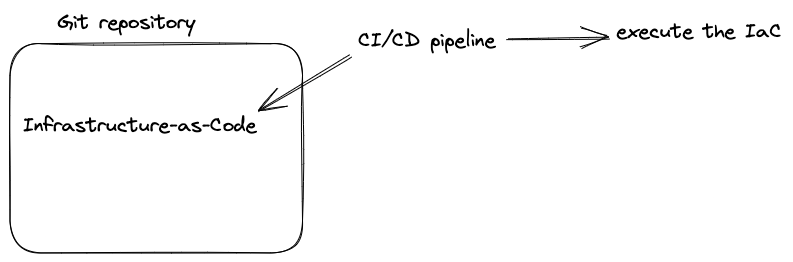
\includegraphics[width=1.00\linewidth]{assets/iac-is-not-gitops.png}
	\caption{IaC is not GitOps.
		%		(\citeauthor{ref}, \citeyear{ref}).
	}
	\label{fig:iacIsNotGitOps}	
\end{figure}

To avoid confusion with what GitOps actually is, 
the OpenGitOps project
\autocite{openGitOpsProject}
was created within the CNCF;
which is maintained by the GitOps working group.

The overall goal of OpenGitOps is to establish a clear vendor-neutral,
principle-driven meaning of GitOps,
which shall provide a foundation for interoperability between tools, conformance and certification through enduring programs, documents and code
\autocite{opengitopsDocuments}.

The definition of GitOps as per the OpenGitOps project
is stated in section \ref{theoretical-background:general-definitions} of this thesis.

In fig. \ref{fig:gitOpsConcept} a visual representation can be seen of the main GitOps concept.

\begin{figure}[h]
	\centering
	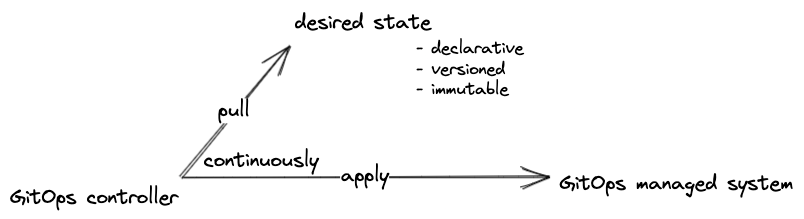
\includegraphics[width=1.00\linewidth]{assets/gitops-concept.png}
	\caption{GitOps concept.
		%		(\citeauthor{ref}, \citeyear{ref}).
	}
	\label{fig:gitOpsConcept}	
\end{figure}







\section{How GitOps changed Continuous Delivery}
\label{theoretical-background:gitops-cd}

Before GitOps, Continuous Delivery was primarliy push-based.
This means that a code change is introduced by a developer,
this code change is commited to a Git repository.
Then a CI/CD system gets triggered to execute a certain pipeline
of jobs.
These jobs may be to test the code and build an artifact, push the artifact
to a registry, etc.
The jobs are run in a pipeline - one after the other -
if one fails, the pipeline is cancelled.
The commit, that is a new version of the code -
is pushed through the pipeline.
Eventually at the end of the pipeline
the new version is deployed by pushing the new artifact
to the deployment environment in an imperative way.
Once the new version is deployed, the pipeline stops.

\begin{figure}[h]
	\centering
	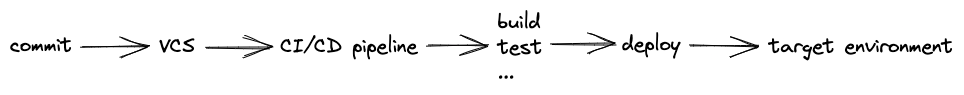
\includegraphics[width=1.00\linewidth]{assets/push-based-cd.png}
	\caption{Push based Continuous Delivery.
		%		(\citeauthor{ref}, \citeyear{ref}).
	}
	\label{fig:pushBasedCD}	
\end{figure}

With GitOps, this primarily push-based process has changed.
Namely, the last couple of steps when the new version
is deployed to the target environment,
are done asynchronously.
With a GitOps workflow,
the CI/CD pipeline usually stops when the new artifact
is successfully pushed to the artifact registry,
or the desired state is changed in the Git repository.
Then another system - the GitOps controller,
which usually lives inside the deployment environment -
notices that the desired state changed and has now
drifted from the actual state.
The GitOps controller then reconciles the new desired state,
by applying it to the managed system.

\begin{figure}[h]
	\centering
	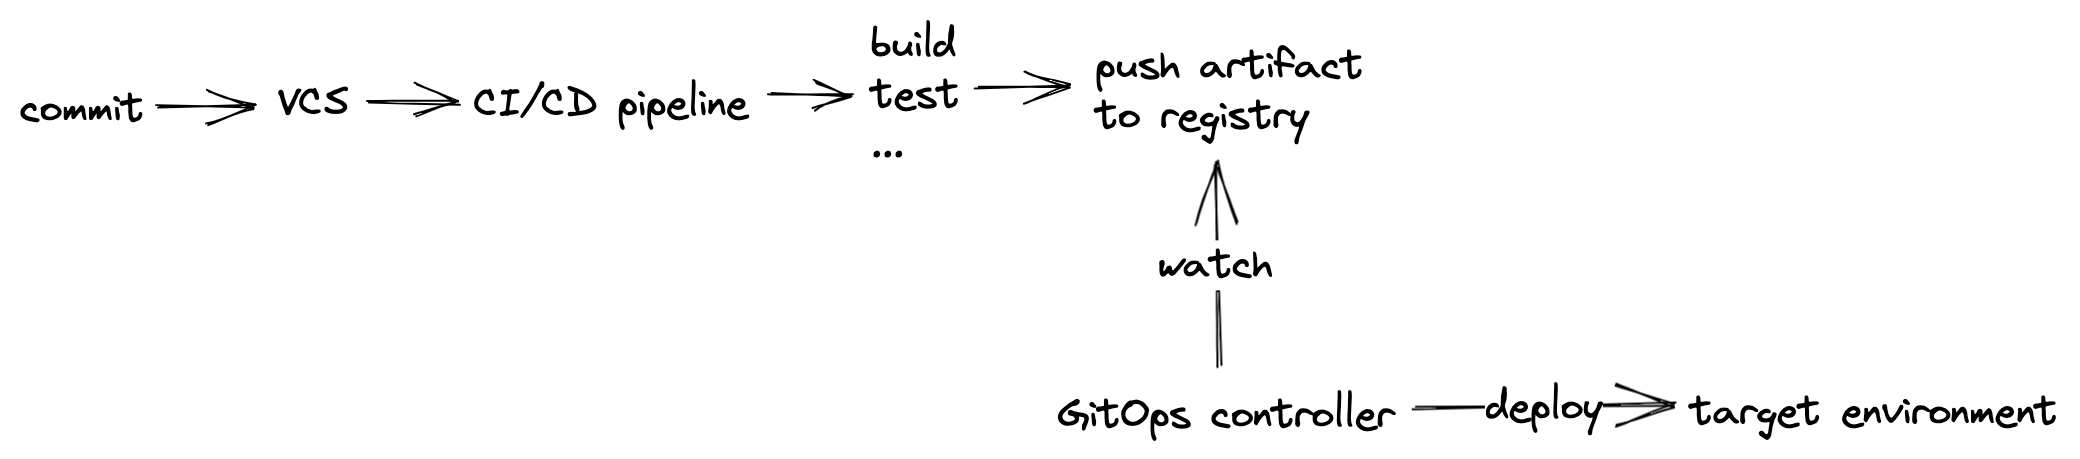
\includegraphics[width=1.00\linewidth]{assets/cd-gitops.png}
	\caption{Continuous Delivery with GitOps.
		%		(\citeauthor{ref}, \citeyear{ref}).
	}
	\label{fig:cd-gitops}	
\end{figure}

One major difference is that with the GitOps workflow,
the CI/CD system no longer knows if and where the application is being
deployed to, since the pipeline usually stops after successful push to the artifact registry.
The desired state, which is stored in a Git repository is continuously being watched
by the GitOps controller. Any changes that it detects are promptly applied to the
target environment.











\section{Promoting Releases Across Environments}

With the push-based pipelines, described in section
\ref{theoretical-background:gitops-cd},
it is typically more straight-forward of how an application
is deployed to multiple target environments.
When the pipeline job to deploy to environment A was successfully done,
the next job to deploy to environment B would be executed.
Since the push-based workflow was a synchronous process from commit
to deployment to target environment,
the whole process could be packed into a single pipeline.

However, with the GitOps workflow the process from
commit to deployment to target environment is usually split up after
publishing of the artifact to the artifact registry.
At this point, the process continues asynchronously.







\section{Towards Progressive Delivery \& Short-Living Environments}

With progressive delivery tools like
Flagger
\autocite{flaggerWebsite}
and
Argo Rollouts
\autocite{argoRolloutsWebsite},
which offer advanced deployment strategies
like canary and blue/green deployments, or A/B testing,
it is now easier to ensure a bad release does not impact the end users
as drastically.
As an example, the named tools make it possible to release new versions
to 10 percent of a specific region of end users,
then this canary rollout is automatically tested and evaluated against metrics,
if certain objectives for metrics fail to be met,
the new release can automatically be rolled back.

\begin{figure}[h]
	\centering
	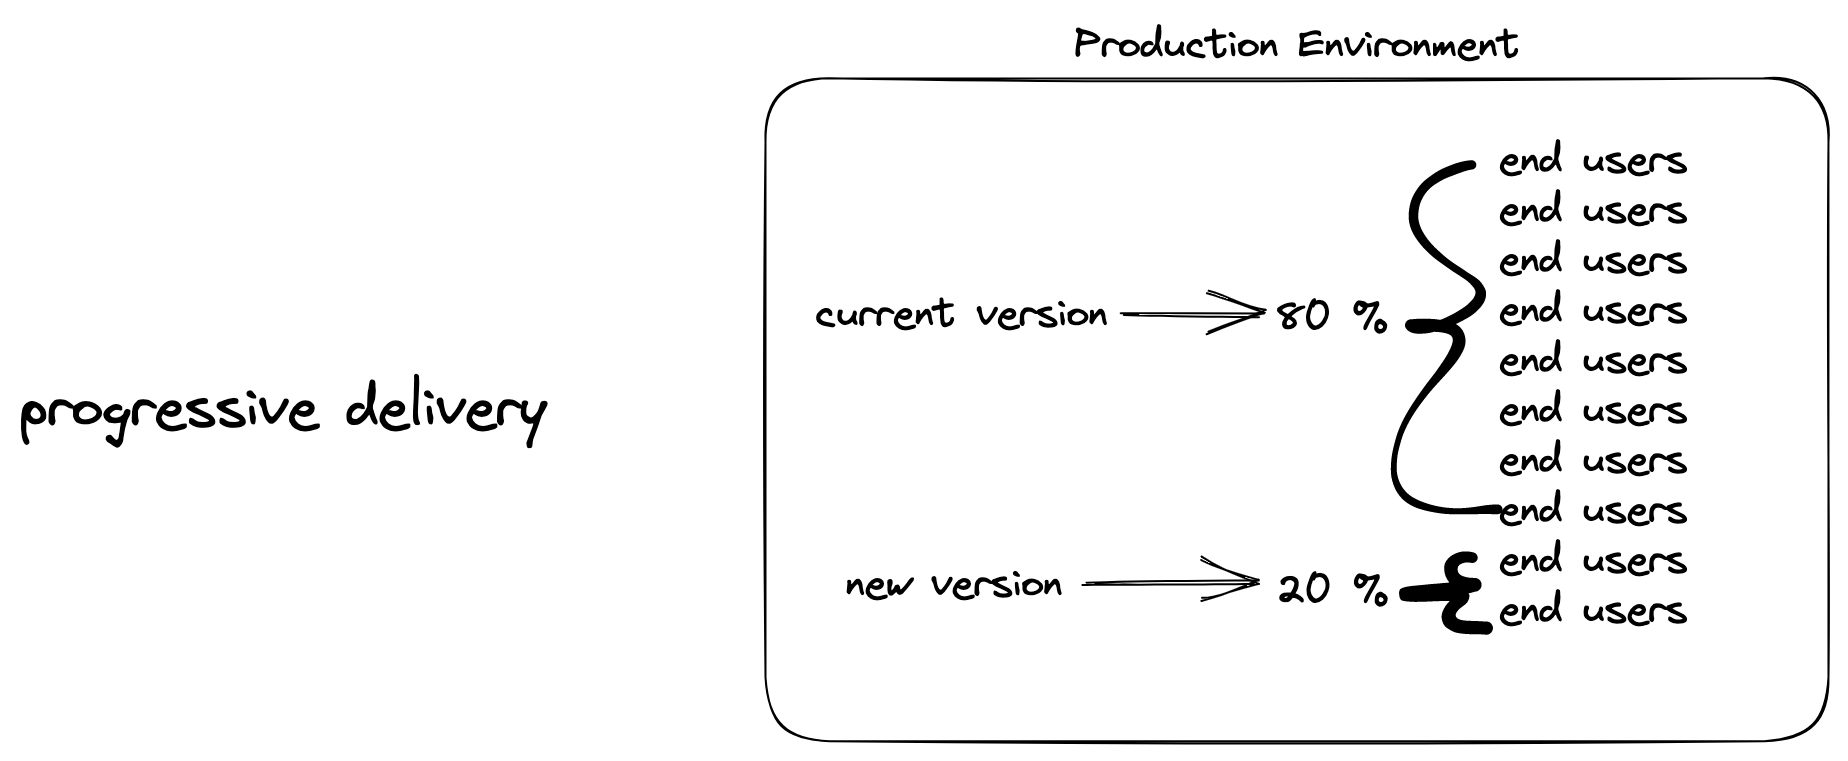
\includegraphics[width=1.00\linewidth]{assets/progressive-delivery.png}
	\caption{Progressive Delivery.
		%		(\citeauthor{ref}, \citeyear{ref}).
	}
	\label{fig:progressive-delivery}	
\end{figure}

Since the progressive delivery tools allow for a more
fine-grained segmentation
of a single environment based on numerous parameters like
client device type, user region, user type (e.g., developer, admin),
registered or unregistered users, etc.
the requirements to have a multitude of deployment environments
have decreased for some organizations.
An illustration can be seen in fig. \ref{fig:progressive-delivery}.

The described segmentation of an environment with the progressive delivery
tools, however might not be possible for every use case or organization.
Financial institutions for example, where the requirement for absolutely zero
errors hitting the production environment is top priority and business critical,
to say the least,
may still want to run multiple environments next to progressive delivery tools,
to ensure an even higher quality and level of caution.
This is illustrated in fig. \ref{fig:deploy-multiple-envs}.

Multiple environments typically mean a big increase in costs;
with progressive delivery the need for multiple environments has decreased,
and this way costs can be reduced.

\begin{figure}[h]
	\centering
	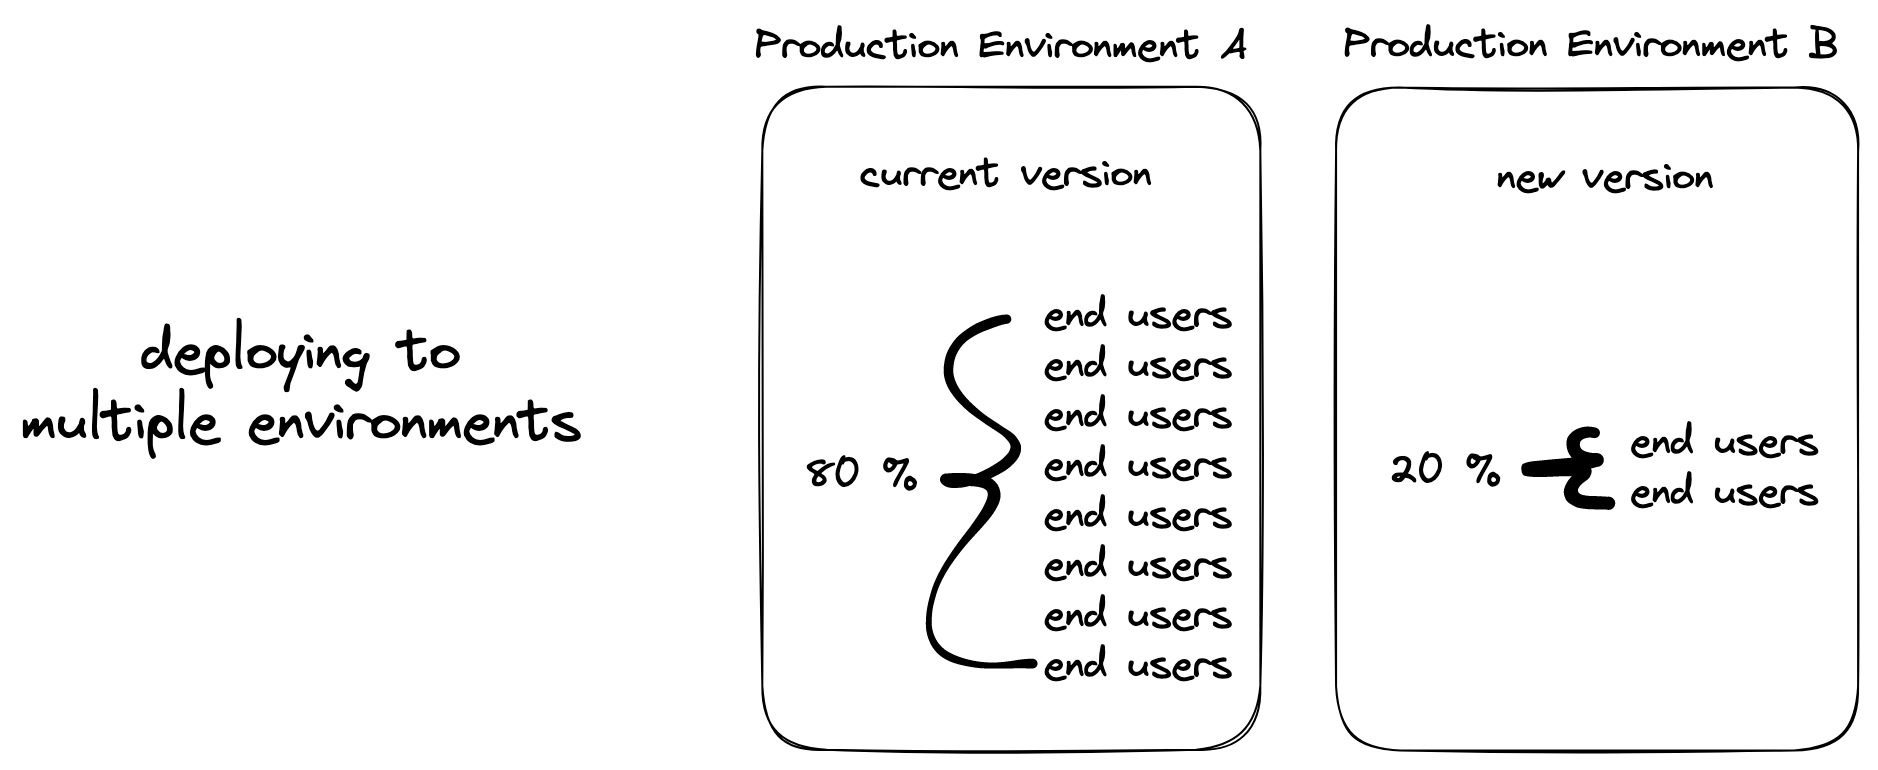
\includegraphics[width=1.00\linewidth]{assets/deploy-multiple-envs.png}
	\caption{Deploying to multiple environments.
		%		(\citeauthor{ref}, \citeyear{ref}).
	}
	\label{fig:deploy-multiple-envs}	
\end{figure}

Nowadays with the rapid development and releasing of new versions,
there has become a need for dynamic, short-living environments.
For every commit of an individual developer,
a deployment environment may be provisioned for previewing the changes
in a live environment that resembles the production environment as well as possible.
This short-living environment may be deleted after a short specified amount of time
has passed.






\section{Beyond container orchestration with Kubernetes}
\label{theoretical-background:kubernetes}

The following section is about
the role Kubernetes plays in the current cloud native ecosystem,
and its extensible architecture.

Since the birth of the cloud native computing foundation (CNCF) in 2015 and the release of Kubernetes as the first CNCF project,
there have emerged more than a hundred projects.
Most of the projects are hosting cloud native technologies and tools to support Kubernetes.
The current ecosystem and toolchains are strongly centered around Kubernetes,
although not strictly tied to it and often times with the explicit effort
for the ability to support alternative cloud native platforms and solutions.

\enquote*{Kubernetes, also known as K8s, is an open-source system for automating deployment, scaling, and management of containerized applications.}
\autocite{kubernetesIoWebsite}
Although this is the primary use case of Kubernetes,
and the reason why it was created initially,
Kubernetes is increasingly being used as a base cloud native platform,
to build other applications and platforms on top of.
The architecture of Kubernetes provides a solid framework and platform,
which is easily extensible.
Developers may extend its API by specifying custom resources and controllers.

There are several advantages when extending the Kubernetes API,
in comparison to a plain REST API.
Some of those are the following
\autocite{kubebuilderBookWebsite}:

\begin{itemize}
	\item \enquote*{Hosted API endpoints, storage, and validation.}
	\item \enquote*{Rich tooling and clis such as kubectl and kustomize.}
	\item \enquote*{Support for Authn and granular Authz.}
	\item \enquote*{Support for API evolution through API versioning and conversion.}
	\item \enquote*{Facilitation of adaptive / self-healing APIs that continuously respond to changes in the system state without user intervention.}
	\item \enquote*{Kubernetes as a hosting environment}
	\autocite{kubebuilderBookWebsite}
\end{itemize}

When developing a Kubernetes-native application,
many of the common capabilities which are often required for all applications,
are being provided by Kubernetes itself, or otherwise easily consumable and integrated.
These may include resource quotas, observability, monitoring, logging and tracing,
configuration state storage, declarative APIs, control loops, and event and message queueing.

\subsection*{Extending Kubernetes}
% https://kubernetes.io/docs/concepts/extend-kubernetes/
Kubernetes offers several different extension points and extension patterns.
Most extension patterns however share the same basic design and principles.
In general, a custom extension is a program which reads and/or writes
to the Kubernetes API. By doing that it can provide useful automation.
Since Kubernetes is based around a declarative API,
where resources are defined as the desired state,
and controllers are responsible for continuously reconciling this
desired state with the actual state,
it has shown to be a good pattern to design custom extensions in the same way
\autocite{extendKubernetes}.

\subsection*{Custom Resources, Controllers and Operators}
% https://kubernetes.io/docs/concepts/architecture/controller/
The concept of a controller and control loop within Kubernetes refers to the
meaning from robotics and automation, where
\enquote*{a control loop is a non-terminating loop that regulates the state of a system.}
\autocite{controllersKubernetes}
Controllers in Kubernetes are continuously running in a control loop,
in specified intervals and sometimes internal or external triggers, 
and watch the actual state of the cluster,
and make changes to it by interacting with the API,
in order to bring the actual state closer to the desired state,
like specified in the declarative definition.
It is typically a good practice to have one controller
be responsible for one resource, 
in order to help with separation of concerns.
Controllers make changes to resources inside the cluster,
like pods and deployments,
but can also be responsible for resources external to the cluster,
like APIs of the infrastructure provider
\autocite{controllersKubernetes}.
A typical controller implementation can be seen in figure
\ref{fig:typicalControllerKubernetes}.
As an example here, the deployment controller continuously ensures the desired state
of three replicas; if it notices the desired state and actual state differ
from one another, it does necessary actions to make them match again.

\begin{figure}[h]
	\centering
	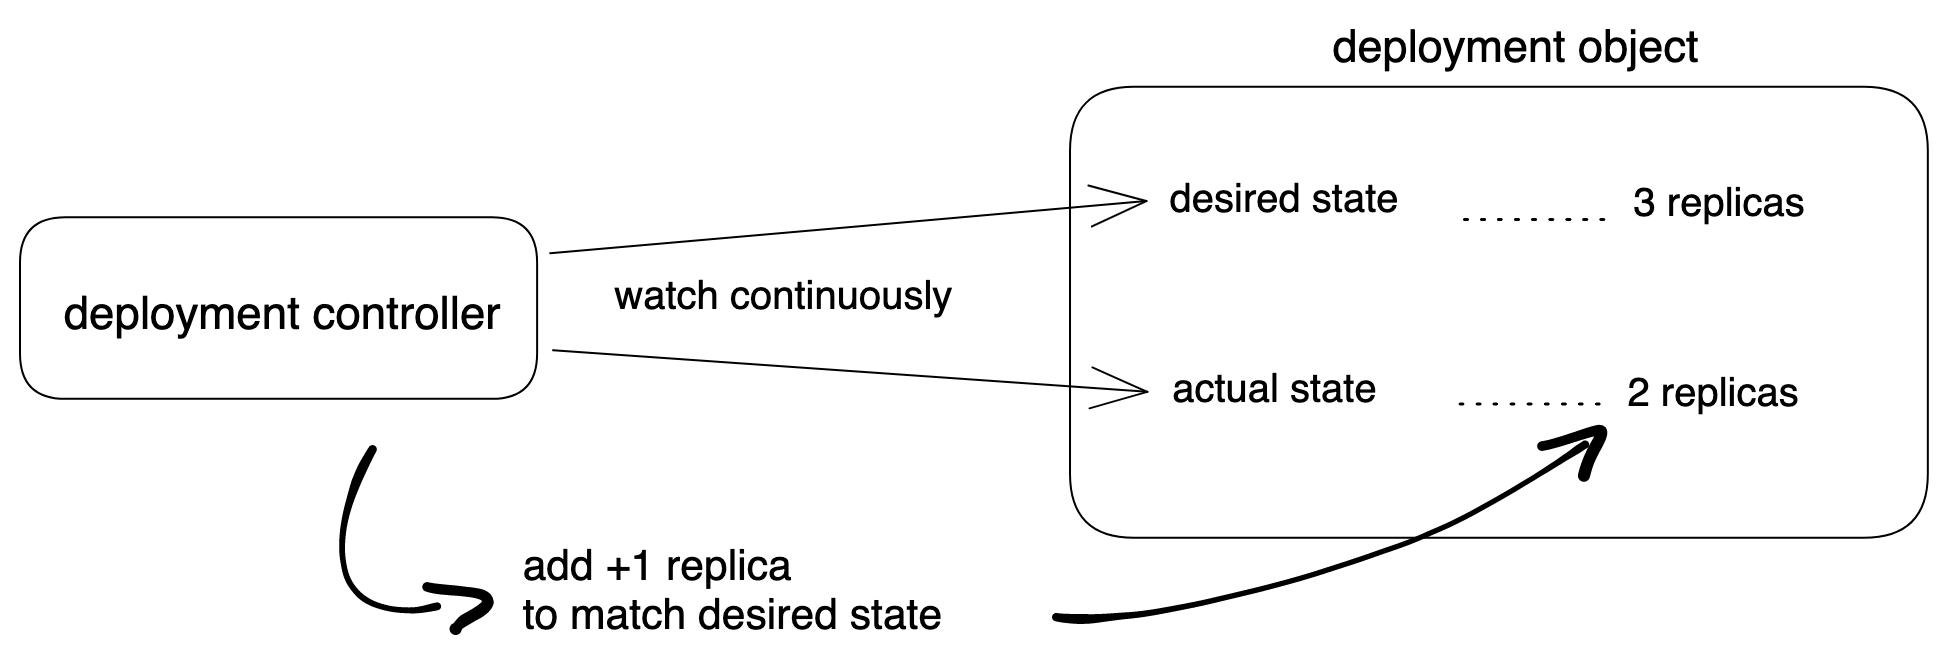
\includegraphics[width=1.00\linewidth]{assets/typical-controller.png}
	\caption{typical controller in Kubernetes.
		%		(\citeauthor{ref}, \citeyear{ref}).
	}
	\label{fig:typicalControllerKubernetes}	
\end{figure}

When a controller has specific domain knowledge,
or does certain tasks, which would usually be done by a human "operator",
it is called an operator.

% https://kubernetes.io/docs/concepts/extend-kubernetes/operator/
Operators typically are a set of controllers and custom resources
with specific codified domain knowledge.
All operational tasks -
which would otherwise have to be done by a human operator -
are written in code.
This code, the controller logic, can then be automated.
Examples for such operational tasks are
backups and restoring of backups, error remediation, database migrations, etc.
\autocite{operatorWhitepaperV1}.
In overly simplified terms:
An operator is a controller plus domain-specific operational knowledge
(fig. \ref{fig:operatorAndController}).

\begin{figure}[h]
	\centering
	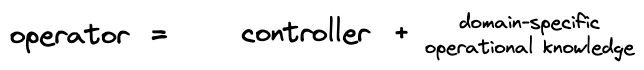
\includegraphics[width=1.00\linewidth]{assets/operator-is-controller-domain-knowledge.png}
	\caption{Operator and Controller.
		%		(\citeauthor{ref}, \citeyear{ref}).
	}
	\label{fig:operatorAndController}	
\end{figure}

The Operator Design Pattern represents a set of principles about
managing complex applications and/or infrastructure resources,
using domain-specific knowledge.
The goal is to limit any manual work that needs to be done,
and try to automate all operational tasks.
This is done by capturing domain-specific knowledge in code,
defining the desired state of resources and exposing them
via a declarative API
\autocite{operatorWhitepaperV1}.

To simplify the process of creating and maintaining Kubernetes-native application
in the form of an operator,
there exist several operator frameworks.
The most prominent framework is the Kubebuilder Framework.
%\url{https://github.com/kubernetes-sigs/kubebuilder}
The Kubebuilder framework makes the process of extending the Kubernetes API
an easy process for developers.
An initial project can easily be boostrapped, allowing the developer to focus
on implementing the custom resource definitions and controller logic.
Any needed Kubernetes primitives, such as service accounts and RBAC permissions
are automatically generated.
Documentation for the OpenAPI resources are also generated from the code,
which is the Go programming language.
There exist rich libraries for interfacing with Kubernetes components,
since Kubernetes itself is also implemented in the Go language
\autocite{kubebuilderBookWebsite}.

With custom resources, the Kubernetes API can dynamically be extended during runtime,
without the need to access its source code or recompile it.

While a resource is
\enquote*{an endpoint in the Kubernetes API that stores a collection of API objects of a certain kind}
\autocite{customResourcesKubernetesIO},
a custom resource is
\enquote*{an extension of the Kubernetes API that is not necessarily available in a default Kubernetes installation}
\autocite{customResourcesKubernetesIO}.
Custom resources can be dynamically registered and independently updated.
Users can interface with its objects as they do with the Kubernetes built-in resources
\autocite{customResourcesKubernetesIO}.









\section{Modeling GitOps Environments}

TODO






\section{Configuration Management Tools}

TODO






\section{GitOps Engines}

TODO








\section{Git Providers}

TODO















\section{Summary}

TODO































%
%\section{Instruction included in the original FHBgld word processor template}
%\subsection{General definitions}
%Die in dieser Formatvorlage beispielhaft enthaltenen Überschriften sind auf die im
%konkreten Fall tatsächlich passenden Überschriften anzupassen.
%In diesem Teil der Arbeit werden die zum eindeutigen Verständnis unbedingt
%erforderlichen Grundlagen und Definitionen sowie die Erklärung wichtiger Begriffe
%angeführt.
%Die Gliederungspunkte müssen möglichst prägnant bezeichnet werden.
%\subsection{Related work / state of research}
%Auch die neuesten Entwicklungen und Arbeiten auf diesem Gebiet (Stand der
%Wissenschaft oder auch state-of-the-art) sind darzulegen, wobei diese je nach Thema
%auch in der 1. Gliederungsebene behandelt werden können.
%
%\section{Ordinary text}
%% A '%' character causes TeX to ignore all remaining text on the line,
%% and is used for comments like this one.
%
%% sections are begun with similar 
%% \subsection and \subsubsection commands.
%
%The ends  of words and sentences are marked by spaces. It doesn't matter how many 
%spaces    you type; one is as good as 100.  The
%end of   a line counts as a space.
%
%One   or more   blank lines denote the  end 
%of  a paragraph.  
%
%Since any number of consecutive spaces are treated
%like a single one, the formatting of the input
%file makes no difference to
%\LaTeX,                % The \LaTeX command generates the LaTeX logo.
%but it makes a difference to you.  When you use 
%\LaTeX \cite{lamport94},  % \cite inserts a reference, which you define at the end of the document
%making your input file as easy to read
%as possible will be a great help as you write 
%your document and when you change it.  This sample 
%file shows how you can add comments to your own input 
%file.
%
%Because printing is different from typewriting,
%there are a number of things that you have to do
%differently when preparing an input file than if
%you were just typing the document directly.
%Quotation marks like
%``this'' 
%have to be handled specially, as do quotes within
%quotes:
%``\,`this'            % \, separates the double and single quote.
%is what I just 
%wrote, not  `that'\,''.  
%
%Dashes come in three sizes: an 
%intra-word 
%dash, a medium dash for number ranges like 
%1--2, 
%and a punctuation 
%dash---like 
%this.
%
%A sentence-ending space should be larger than the
%space between words within a sentence.  You
%sometimes have to type special commands in
%conjunction with punctuation characters to get
%this right, as in the following sentence.
%Gnats, gnus, etc.\ all  % `\ ' makes an inter-word space.
%begin with G\@.         % \@ marks end-of-sentence punctuation.
%You should check the spaces after periods when
%reading your output to make sure you haven't
%forgotten any special cases.  Generating an
%ellipsis
%\ldots\               % `\ ' is needed after `\ldots' because TeX 
%% ignores spaces after command names like \ldots 
%% made from \ + letters.
%%
%% Note how a `%' character causes TeX to ignore 
%% the end of the input line, so these blank lines 
%% do not start a new paragraph.
%%
%with the right spacing around the periods requires
%a special command.
%
%\LaTeX\ interprets some common characters as
%commands, so you must type special commands to
%generate them.  These characters include the
%following:
%\$ \& \% \# \{ and \}.
%
%In printing, text is usually emphasized with an
%\emph{italic}  
%type style.  
%
%\begin{em}
%	A long segment of text can also be emphasized 
%	in this way.  Text within such a segment can be 
%	given \emph{additional} emphasis.
%\end{em}
%
%It is sometimes necessary to prevent \LaTeX\ from
%breaking a line where it might otherwise do so.
%This may be at a space, as between the ``Mr.''\ and
%``Jones'' in
%``Mr.~Jones'',        % ~ produces an unbreakable interword space.
%or within a word---especially when the word is a
%symbol like
%\mbox{\emph{itemnum}} 
%that makes little sense when hyphenated across
%lines.
%
%Footnotes\footnote{This is an example of a footnote.}
%pose no problem.
%
%\LaTeX\ is good at typesetting mathematical formulas
%like
%\( x-3y + z = 7 \) 
%or
%\( a_{1} > x^{2n} + y^{2n} > x' \)
%or  
%\( AB  = \sum_{i} a_{i} b_{i} \).
%The spaces you type in a formula are 
%ignored.  Remember that a letter like
%$x$                   % $ ... $  and  \( ... \)  are equivalent
%is a formula when it denotes a mathematical
%symbol, and it should be typed as one.
%Furthermore you can add a formula as Images or Tables, see Formula  \hyperref[eq:abc]{\ref{eq:abc}}
%\begin{equation}
%	\label{eq:abc}
%	a+b=c
%\end{equation}
%
%It is sometimes necessary to prevent \LaTeX\ from
%breaking a line where it might otherwise do so.
%This may be at a space, as between the ``Mr.''\ and
%``Jones'' in
%``Mr.~Jones'',        % ~ produces an unbreakable interword space.
%or within a word---especially when the word is a
%symbol like
%\mbox{\emph{itemnum}} 
%that makes little sense when hyphenated across
%lines.
